\chapter{Teoretické pozadí}

\section{Umělá inteligence v deskových hrách}

Deskové hry představují jednu z tradičních oblastí výzkumu umělé inteligence. Díky jasným pravidlům, 
deterministickým charakteristikám a jednoznačně určeným podmínkám vítězství poskytují perfektní prostředí
pro testování algoritmů z oblasti umělé inteligence. Výzkum v této oblasti přispěl k rozvoji metod pro prohledávání
stavového prostoru i moderních přístupů strojového učení \cite{russell2021aima}.

Většina zkoumaných deskových her patří mezi deterministické s úplnou informací. To znamená, že oba hráči mají 
přístup ke stejným informacím o stavu hry a pravidly je jasně dané, jak každá akce stav změní. Díky těmto 
vlastnostem lze průběh partie velmi dobře modelovat jako prohledávání herního stavového prostoru, který 
je tvořen právě danými herními pozicemi \cite{russell2021aima}.

Přestože se může zdát, že díky jasně daným pravidlům je řešení herního stavového prostoru jednoduché, tak 
v realitě tomu tak bohužel není. Počet možných pozic roste se složitostí hry natolik, že úplné prohledávání
herního stromu je prakticky nemožné. Tento problém vedl k vývoji algoritmů, které jsou schopné vybírat dobré tahy
bez nutnosti procházet všechny možné pokračování partie \cite{russell2021aima,browne2012mcts}.

Mezi nejvýznamnější přístupy používané při rozhodování v deskových hrách patří algoritmy založené na prohledávání herního stromu.
Následující sekce představuje základní principy takových algoritmů, jako je minimax a alfa-beta ořezávání, které tvoří pevný
základ pro mnoho moderních metod pro rozhodování \cite{russell2021aima,browne2012mcts}.

\section{Prohledávání herních stromů}

Průběh každé deskové hry lze reprezentovat pomocí herního stromu. Vrcholy stromu představují stavy hry a hrany odpovídají 
legálním tahům, které jsou z pravidel jasně dané. Takovým tahem jsme tedy schopni přejít z dosavadního stavu do dalšího
validního stavu. Kořenem stromu je aktuální pozice (na začátku hry tedy původní pozice dle pravidel) a listy stromu představují
koncové stavy, tedy jinými slovy vítězství jednoho z hráčů nebo remízu \cite{russell2021aima}.

Ve většině netriviálních her je množství validních tahů, tudíž i následujících stavů, natolik vysoké, že úplné prohledávání stromu
je výpočetně nemožné. S rostoucí hloubkou stromu roste počet stavů exponenciálně, což vede k příliš náročným výpočetním požadavkům \cite{russell2021aima}.

Cílem moderních algoritmů pro prohledávání stavového prostoru proto není projít všechny herní stavy co nejrychleji, ale efektivně 
nalézt, případně vybrat, takové tahy, které maximalizují šanci na vítězství pro daného hráče při omezeném výpočetním čase. 
Algoritmy se především liší způsobem výběru větví stromu a také metodou jejich vyhodnocování.

Mezi nejznámější algoritmy využívající tento princip patří minimax a jeho případná optimalizace pomocí alfa-beta 
ořezávání. Tyto metody tvoří základ pro klasické přístupy k rozhodování v deskových hrách a slouží jako výchozí
bod pro modernější algoritmy, jako například MCTS \cite{russell2021aima,browne2012mcts}.

\begin{figure}[H]
    \centering
    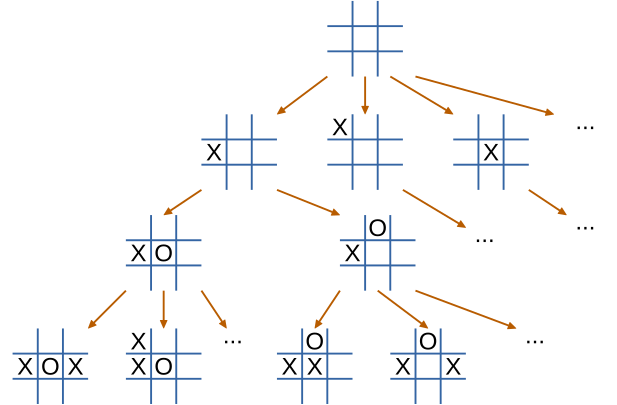
\includegraphics[width=0.8\textwidth]{img/tic_tac_toe.png}
    \caption{Příklad části herního stromu pro hru Tic-Tac-Toe. Převzato z \cite{dingle2019notes}.}
    \label{fig:game_tree}
\end{figure}

\subsection{Minimax}
\label{sec:minimax}

Algoritmus minimax je jeden ze základních algoritmů pro rozhodování v deterministických hrách s úplnou informací.
Cílem je nalézt tah, který maximalizuje šanci na vítězství pro hráče na tahu za předpokladu, že soupeř vždy zvolí 
optimální odpověď. Algoritmus tedy vychází z předpokladu racionálního protihráče, nikoli náhodného nebo chybujícího \cite{russell2021aima}.

Základním předpokladem algoritmu tedy je, že se partie odehrává mezi dvěma racionálními hráči s opačnými cíli. Jeden z hráčů, označovaný jako MAX,
se snaží maximalizovat hodnotu výsledné pozice, zatímco druhý hráč, označovaný jako MIN, se snaží tuto hodnotu minimalizovat. Hodnota pozice je číselné
ohodnocení stavu z pohledu hráče MAX, kdy vyšší hodnota odpovídá lepší pozici pro tohoto hráče \cite{russell2021aima}.

Při průchodu stromem tedy algoritmus střídavě uvažuje tahy obou hráčů. Ve vrcholech, které odpovídají tahům hráče MAX je z možných pokračování 
vybrána větev s nejvyšší hodnotou. Naopak ve vrcholech, kdy je na tahu hráč MIN je zvolena větev s nejnižší možnou hodnotou, jelikož se 
předpokládá, že soupeř hraje optimálně a tudíž se hráči MAX snaží zabránit v dosažení co nejlepšího výsledku. Tímto způsobem se hodnoty vrcholů 
postupně propagují od listů stromu směrem ke kořeni. V koncových stavech bývá hodnota pozice obvykle definována jako $1$ pro vítězství hráče MAX, 
$0$ pro remízu a $-1$ pro vítězství hráče MIN. Po propagaci těchto hodnot až ke kořeni stromu lze určit optimální tah \cite{russell2021aima}.

Výpočet algoritmu minimax probíhá rekurzivním průchodem herního stromu. Algoritmus nejprve sestoupí až do listů nebo do předem stanovené
hloubky prohledávání. Následně začne postupně vyhodnocovat jednotlivé pozice a jejich hodnoty pak propaguje směrem ke kořeni stromu. Každý vnitřní 
vrchol je ohodnocen na základě hodnot svých potomků podle toho, zda se jedná o tah hráče MAX nebo MIN. Ve vrcholech hráče MAX je výsledná hodnota 
určena jako maximum z hodnot všech bezprostředních následníků. Naopak ve vrcholech hráče MIN je zvolena nejmenší hodnota z dostupných pokračování.
Tento postup je opakován rekurzivně, dokud není ohodnocen také kořen stromu. Hodnota kořenového vrcholu následně určuje nejlepší tah, který má hráč 
MAX v dané pozici k dispozici \cite{russell2021aima}.

Princip algoritmu lze formálně popsat pomocí rekurzivní hodnoticí funkce, která každému vrcholu herního stromu přiřadí hodnotu odpovídající
nejlepšímu výsledku dosažitelnému z dané pozice.

\[
V(s)=
\begin{cases}
\max\limits_{s' \in Succ(s)} V(s'), & \text{je-li } s \text{ vrchol hráče MAX},\\[1ex]
\min\limits_{s' \in Succ(s)} V(s'), & \text{je-li } s \text{ vrchol hráče MIN},\\[1ex]
Eval(s), & \text{je-li } s \text{ list nebo dosažená maximální hloubka.}
\end{cases}
\]

Funkce $V(s)$ představuje výslednou hodnotu pozice s. Množina $Succ(s)$ označuje všechny bezprostřední následníky daného vrcholu, 
tedy pozice dosažitelné jedním legálním tahem. Ve vrcholech hráče MAX je z hodnot následníků vybráno maximum, naopak ve vrcholech
hráče MIN minimum. Pokud algoritmus dosáhne listu nebo předem stanovené maximální hloubky prohledávání, je hodnota pozice
určena pomocí hodnoticí funkce $Eval(s)$. V nejjednodušším případě může tato funkce vracet hodnoty $1$, $0$ a $-1$, které odpovídají výhře hráče MAX,
remíze a výhře hráče MIN. Ve složitějších hrách však bývá nahrazena heuristickou nebo naučenou ohodnocovací funkcí, která umožní odhadnout
kvalitu dosaženého stavu bez prohledání stromu až do konce \cite{russell2021aima}.

Samotný algoritmus lze zapsat rekurzivně. Na vstupu dostává aktuální stav hry a informaci o tom, zda je na tahu hráč MAX nebo MIN. Pokud 
je dosažen koncový stav nebo maximální hloubka prohledávání, algoritmus vrátí hodnotu dané pozice pomocí funkce $Eval$. V opačném případě 
rekurzivně vyhodnotí všechny následníky a podle hráče na tahu vybere maximum nebo minimum.

\begin{algorithm}[H]
\caption{Algoritmus minimax}
\label{alg:minimax}
\begin{algorithmic}[1]
\Function{Minimax}{$s, depth, maximizingPlayer$}
    \If{$s$ je koncový stav nebo $depth = 0$}
        \State \Return $Eval(s)$
    \EndIf

    \If{$maximizingPlayer$}
        \State $best \gets -\infty$
        \ForAll{$s' \in Succ(s)$}
            \State $best \gets \max(best, \Call{Minimax}{s', depth - 1, false})$
        \EndFor
        \State \Return $best$
    \Else
        \State $best \gets +\infty$
        \ForAll{$s' \in Succ(s)$}
            \State $best \gets \min(best, \Call{Minimax}{s', depth - 1, true})$
        \EndFor
        \State \Return $best$
    \EndIf
\EndFunction
\end{algorithmic}
\end{algorithm}

Parametr $depth$ omezuje hloubku prohledávání a umožňuje algoritmus použít i v případech, kdy je strom moc velký a  není možné ho prohledat celý
až do koncových stavů. Proměnná $maximizingPlayer$ určuje, zda se aktuální vrchol vyhodnocuje z pohledu hráče MAX nebo MIN. Funkce 
$Succ(s)$ vrací všechny stavy dosažitelné z pozice $s$ jedním legálním tahem.

Přestože algoritmus minimax zaručuje nalezení optimálního tahu při předpokladu optimální hry obou hráčů, jeho hlavní nevýhodou je vysoká výpočetní
složitost. V nejhorším případě musí algoritmus navštívit všechny vrcholy herního stromu až do hloubky prohledávání. Časová složitost algoritmu
je proto $O(b^d)$, kde $b$ představuje průměrný faktor větvení a $d$ hloubku prohledávání. Paměťová složitost při implementaci pomocí rekurzivního průchodu 
odpovídá $O(d)$, protože je v paměti současně uložena pouze aktuálně procházená větev stromu \cite{russell2021aima}.

Hlavní výhodou algoritmu minimax je jeho jednoduchost a schopnost nalézt optimální tah. 
Díky tomu představuje základ mnoha dalších algoritmů používaných při rozhodování v deskových hrách. Jeho zásadní nevýhodou je však 
exponenciální časová složitost, která prakticky znemožňuje použití úplného prohledávání u složitějších her. V praxi je proto algoritmus 
často kombinován s omezenou hloubkou prohledávání, heuristickými hodnoticími funkcemi nebo dalšími optimalizacemi.

Právě takovou optimalizací algoritmu minimax je alfa-beta ořezávání. Tato metoda umožňuje během prohledávání vynechat 
části herního stromu, které nemohou ovlivnit výsledné rozhodnutí. Výsledkem je výrazné snížení počtu navštívených vrcholů při 
zachování stejného výsledného tahu jako u klasického algoritmu minimax \cite{russell2021aima}.


\subsection{Alfa-beta ořezávání}
\label{sec:pruning}

Přestože algoritmus minimax zaručuje nalezení optimálního tahu, jeho praktické využití je výrazně omezeno vysokou časovou složitostí. 
Ve většině deskových her není možné prohledat celý herní strom do dostatečné hloubky během rozumného času pouze s použitím algoritmu  minimax. 
Z tohoto důvodu vznikla řada optimalizačních metod, jejichž cílem je snížit počet navštívených vrcholů bez ovlivnění výsledného rozhodnutí. 
Nejvýznamnější z nich je právě algoritmus alfa-beta ořezávání, který dokáže vynechat části herního stromu, jejichž prohledání 
nemůže mít vliv na konečnou volbu tahu \cite{russell2021aima}.

Algoritmus alfa-beta ořezávání využívá skutečnosti, že během prohledávání stromu lze u některých větví již před jejich úplným prozkoumáním 
rozhodnout, zda mohou či nemohou ovlivnit výslednou hodnotu nadřazeného vrcholu. Za tímto účelem algoritmus udržuje dvě krajní hodnoty označované jako
$\alpha$  a $\beta$. Hodnota $\alpha$  představuje nejlepší dosud nalezenou hodnotu pro hráče MAX, zatímco $\beta$  odpovídá nejlepší hodnotě dosažitelné
pro hráče MIN. Tyto hodnoty jsou průběžně aktualizovány během rekurzivního průchodu stromem \cite{russell2021aima}.

Během průchodu herním stromem jsou hodnoty $\alpha$ a $\beta$ průběžně aktualizovány podle dosud nalezených výsledků. Pokud v určitém okamžiku nastane
situace, kdy je hodnota $\alpha$ větší nebo rovna hodnotě $\beta$, lze zbývající následníky aktuálního vrcholu bezpečně vynechat. Jejich prohledání
totiž nemůže mít vliv na výslednou hodnotu žádného z nadřazených vrcholů, a tudíž ani konečné rozhodnutí. Tento proces se označuje jako 
alfa-beta ořezávání a představuje hlavní metodu úspory výpočetního času \cite{russell2021aima}.

\begin{figure}[H]
    \centering
    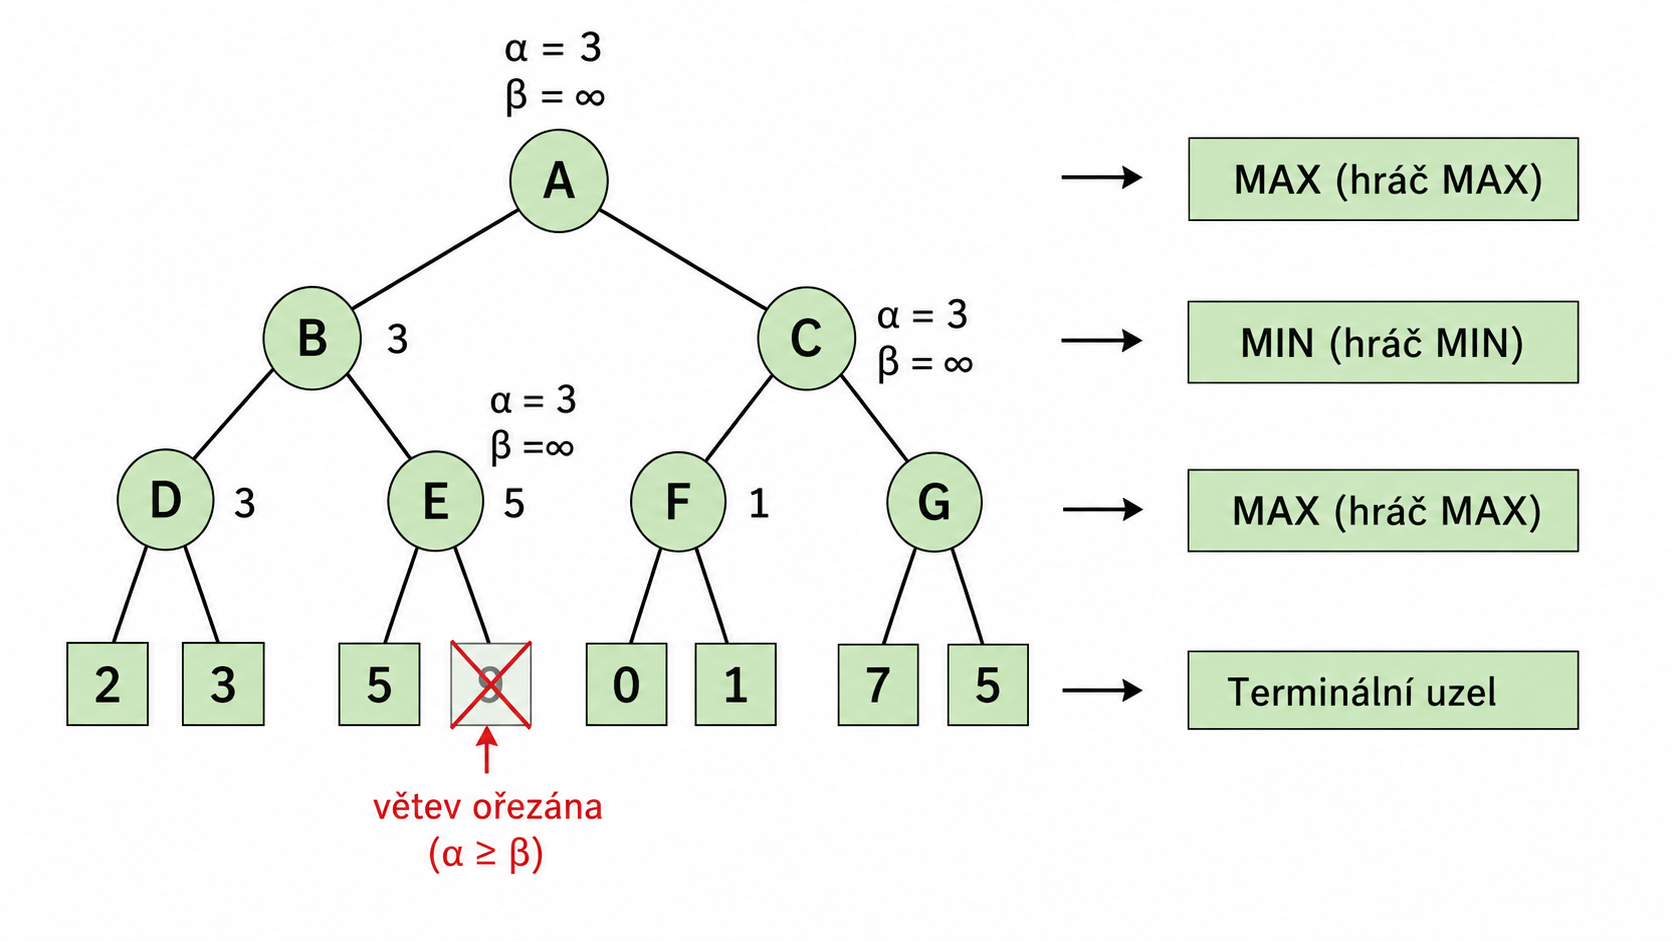
\includegraphics[width=0.85\textwidth]{img/alpha-beta-tree.png}
    \caption{Příklad průběhu alfa-beta ořezávání. Větev označená červeně není dále prohledávána, protože nemůže ovlivnit výsledné rozhodnutí algoritmu.}
    \label{fig:alpha_beta}
\end{figure}

Algoritmus alfa-beta ořezávání se od klasického algoritmu minimax liší především tím, že během rekurzivního průchodu 
stromem udržuje mezní hodnoty $\alpha$ a $\beta$. Jakmile je splněna podmínka $\alpha \geq \beta$, lze zbývající 
větve aktuálního vrcholu bezpečně vynechat, protože již nemohou ovlivnit výsledné rozhodnutí.

\begin{algorithm}[H]
\caption{Algoritmus alfa-beta ořezávání}
\label{alg:alphabeta}
\begin{algorithmic}[1]
\Function{AlphaBeta}{$s, depth, \alpha, \beta, maximizingPlayer$}
    \If{$s$ je koncový stav nebo $depth = 0$}
        \State \Return $Eval(s)$
    \EndIf

    \If{$maximizingPlayer$}
        \State $value \gets -\infty$
        \ForAll{$s' \in Succ(s)$}
            \State $value \gets \max(value,\Call{AlphaBeta}{s', depth-1,\alpha,\beta,false})$
            \State $\alpha \gets \max(\alpha,value)$
            \If{$\alpha \geq \beta$}
                \State \textbf{break}
            \EndIf
        \EndFor
        \State \Return $value$
    \Else
        \State $value \gets +\infty$
        \ForAll{$s' \in Succ(s)$}
            \State $value \gets \min(value,\Call{AlphaBeta}{s', depth-1,\alpha,\beta,true})$
            \State $\beta \gets \min(\beta,value)$
            \If{$\alpha \geq \beta$}
                \State \textbf{break}
            \EndIf
        \EndFor
        \State \Return $value$
    \EndIf
\EndFunction
\end{algorithmic}
\end{algorithm}

Na rozdíl od algoritmu minimax jsou během výpočtu udržovány dvě mezní hodnoty, $\alpha$ a $\beta$,
které reprezentují dosud nejlepší nalezené výsledky pro hráče MAX a MIN. Jakmile je splněna podmínka
$\alpha \geq \beta$, zbývající následníci aktuálního vrcholu již nemohou ovlivnit výsledné rozhodnutí 
a jejich prohledávání je ukončeno.

Přestože alfa-beta ořezávání v nejhorším případě navštíví stejný počet vrcholů jako algoritmus minimax,
v praxi dokáže počet prohledaných stavů výrazně snížit. Nejhorší časová složitost proto zůstává $O(b^d)$, avšak 
při ideálním pořadí prohledávání větví lze dosáhnout složitosti přibližně $O(b^{d/2})$. To v praxi umožňuje prohledat
výrazně větší hloubku stromu při stejném výpočetním čase \cite{russell2021aima}.

Hlavní výhodou alfa-beta ořezávání je zachování stejného výsledku jako u algoritmu minimax se současným snížením 
počtu navštívených vrcholů. Úspěšnost ořezávání však výrazně závisí na pořadí, ve kterém jsou jednotlivé tahy prohledávány.
Čím dříve algoritmus nalezne kvalitní tahy, tím více větví bude ořezáno. Z tohoto důvodu jsou v moderních implementacích
často využívány heuristiky pro řazení tahů ještě před samotným prohledáváním \cite{russell2021aima}.

Přestože alfa-beta ořezávání představuje významné zrychlení algoritmu minimax, u her s velmi vysokým faktorem větvení nebo velmi
rozsáhlým stavovým prostorem přestává být i tento přístup efektivní. V takových případech se stále častěji využívají metody
založené na selektivním prohledávání herního stromu. Jednou z nejúspěšnějších metod tohoto typu je MCTS,
který místo systematického prohledávání využívá řízené simulace a statistické vyhodnocování navštívených stavů \cite{browne2012mcts}.

\section{Monte Carlo Tree Search}
\label{sec:mcts}

\subsection{Motivace}

Přestože algoritmus minimax spolu s alfa-beta ořezáváním představuje efektivní řešení pro mnoho klasických deskových her, tak
existují hry, u kterých tyto metody zkrátka přestávají být v praxi použitelné. Důvodem je hlavně velmi vysoký faktor větvení a 
rozsáhlý stavový prostor, které znemožňují prohledání dostatečně hluboké části herního stromu v rozumném čase. Typickým příkladem
takové hry je Go, jejíž počet možných pozic i tahů výrazně převyšuje možnosti klasických algoritmů založených na úplném prohledávání 
stromu \cite{browne2012mcts}.

Potřeba efektivnějšího prohledávání rozsáhlejších herních stromů vedla ke vzniku algoritmu Monte Carlo Tree Search (MCTS), který se během
posledních pár desetiletí stal jedním z nejvýznamnějších algoritmů pro rozhodování v deskových hrách a dalších sekvenčních rozhodovacích
úlohách \cite{browne2012mcts}.

\subsection{Základní princip}

Na rozdíl od algoritmů minimax nebo alfa-beta neprohledává MCTS všechny možné větve herního stavového stromu. 
Namísto toho se soustředí zejména na větve, které se podle dosavadních simulací jeví jako nejvhodnější. Algoritmus
tedy postupně buduje pouze část herního stromu, jehož velikost se zvětšuje s rostoucím počtem simulací.

Každá iterace algoritmu se skládá ze čtyř na sebe navazujících fází: Selekce (Selection), Rozšíření (Expansion), Simulace (Simulation) 
a zpětná propagace(Backpropagation).
Během těchto fází algoritmus vybere vhodnou větev stromu, rozšíří ji o nový vrchol, provede simulaci průběhu hry a získaný 
výsledek zpětně propaguje ke kořeni stromu. Opakováním tohoto procesu algoritmus postupně zpřesňuje odhad kvality jednotlivých tahů \cite{browne2012mcts}.

\subsection{Čtyři fáze algoritmu}

\begin{figure}[H]
    \centering
    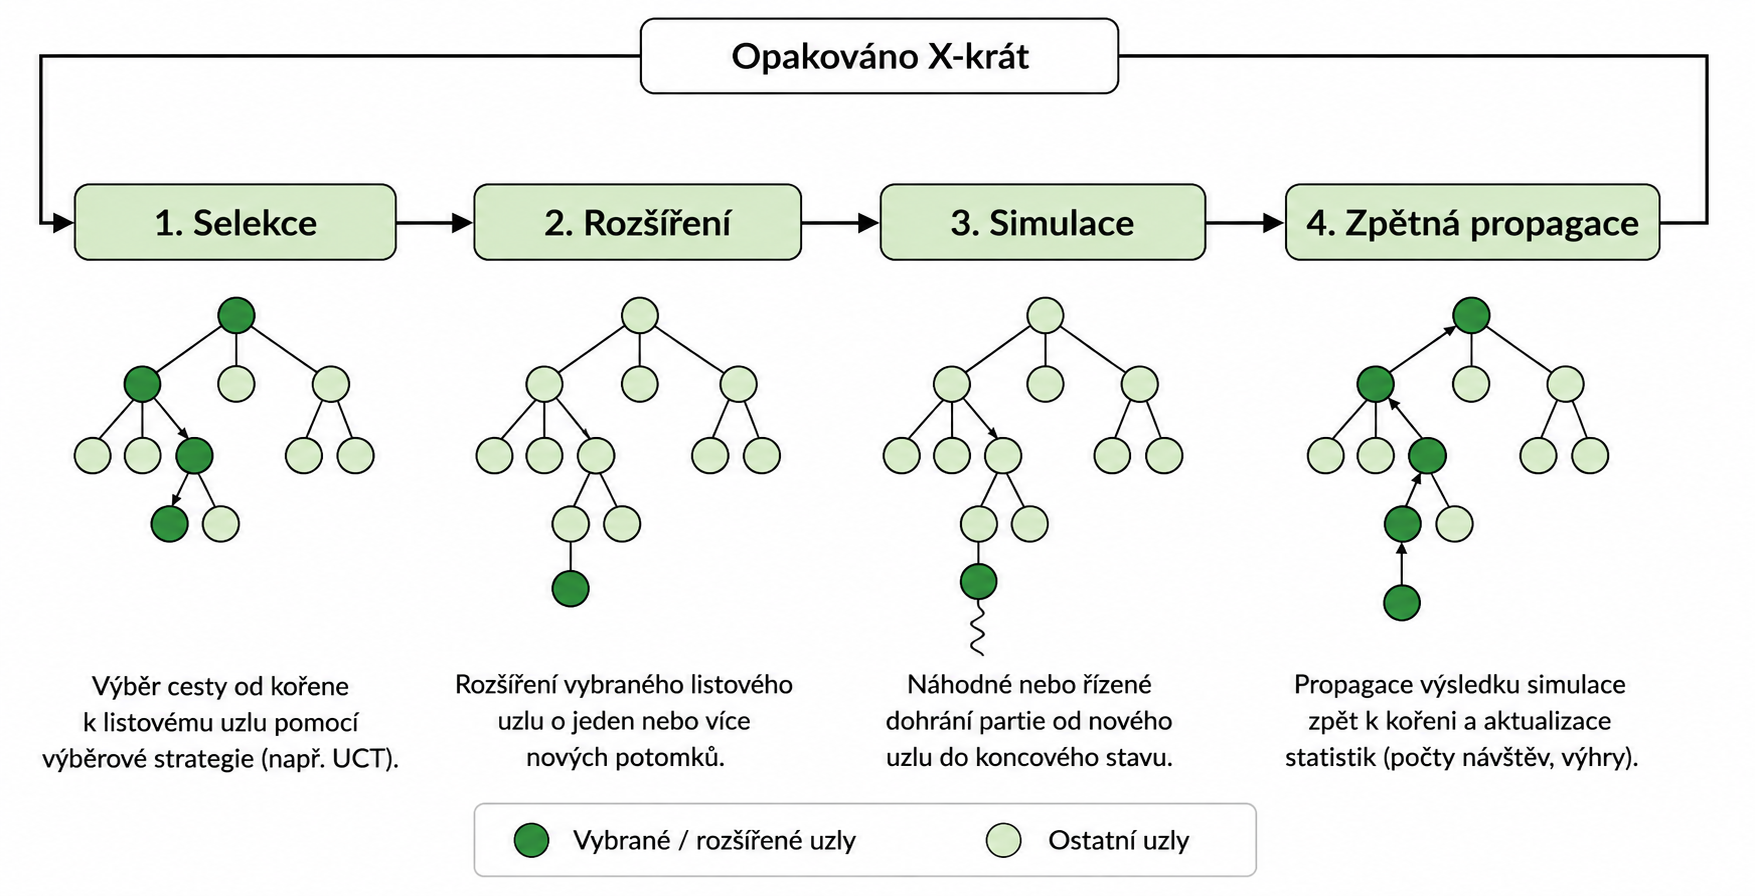
\includegraphics[width=\textwidth]{img/MCTS-phases.png}
    \caption{Jedna iterace algoritmu Monte Carlo Tree Search. Algoritmus opakovaně provádí čtyři základní fáze: selekci,
     rozšíření, simulaci a zpětnou propagaci. Převzato a upraveno podle \cite{geeksforgeeks_mcts}.}
    \label{fig:mcts_phases}
\end{figure}

\subsubsection{Selekce}

Cílem fáze selekce je zvolit cestu od kořene herního stromu k některému z již existujících listových vrcholů,
který bude dále rozšířen. Algoritmus při tomto průchodu v každém vrcholu vybírá jednoho ze svých potomků podle
strategie založené na statistikách získaných z předchozích simulací. Výsledkem této fáze je nalezení 
uzlu, ve kterém bude strom dále rozšířen o nové pokračování partie \cite{browne2012mcts}.

Smyslem selekce není pouze opakovaně navštěvovat dosud nejúspěšnější větve stromu. Naopak je nutné nalézt rovnováhu 
mezi využitím již prozkoumaných kvalitních tahů a objevováním nových možností, které zatím nebyly dostatečně prozkoumány. 
Tento kompromis je označován jako \emph{exploitation} a \emph{exploration} a představuje jednu z klíčových myšlenek algoritmu MCTS. 
Samotná výběrová strategie bývá nejčastěji realizována pomocí algoritmu UCT. \cite{browne2012mcts,kocsis2006uct}.

Výsledkem fáze selekce je nalezení listového uzlu, který bude v následující fázi rozšířen.

\subsubsection{Rozšíření}

Jakmile je během selekce nalezen vhodný listový uzel, následuje ho fáze rozšíření. Jejím cílem je přidat do herního stromu 
nový vrchol odpovídající některému z dosud neprozkoumaných legálních tahů. Tím dochází k postupnému rozšiřování stromu o 
nové části stavového prostoru, které dosud nebyly navštíveny \cite{browne2012mcts}.

Ve většině implementací není při jedné iteraci rozšířeno více uzlů, ale pouze jeden nový následník vybraného vrcholu. Nově 
vytvořený uzel následně slouží jako výchozí bod pro fázi simulace, během které je odhadnuta kvalita odpovídající pozice. 
Postupným opakováním tohoto procesu algoritmus rozšiřuje herní strom pouze v oblastech, které byly během selekce vyhodnoceny 
jako kvalitní \cite{browne2012mcts}.

Výsledkem fáze rozšíření je přidání nového uzlu do herního stromu, ze kterého je následně provedena simulace průběhu hry.

\subsubsection{Simulace}

Po fázi rozšíření následuje simulace, jejímž cílem je odhadnout kvalitu přidaného uzlu. V základní podobě 
algoritmu MCTS je ze stavu odpovídajícího tomuto uzlu spuštěna simulovaná partie, která pokračuje až do koncového
stavu. Tahy během simulace mohou být vybírány náhodně nebo podle jednoduché strategie. Výsledkem simulace je 
hodnota, která vyjadřuje, zda daná partie skončila výhrou, prohrou nebo remízou z pohledu hráče, pro kterého je strom vyhodnocován \cite{browne2012mcts}.

Simulace tedy nahrazuje úplné systematické prohledávání stromu statistickým odhadem. Jedna simulace sama o sobě nemusí 
poskytovat přesný odhad kvality pozice, ale při velkém počtu opakování se výsledky jednotlivých simulací postupně zprůměrují 
a umožňují rozlišit mezi více slibnými a méně slibnými tahy. Právě tato vlastnost umožňuje MCTS algoritmu pracovat i v nadrozměrných 
stavových prostorech, kde by úplné prohledávání nebylo možné.

Výsledkem fáze simulace je ohodnocení nově prozkoumané pozice, které je v následující fázi zpětně propagováno až ke kořeni stromu.

\subsubsection{Zpětná propagace}

Po dokončení simulace následuje fáze zpětné propagace. Během ní je výsledek simulované partie přenesen zpět po cestě, která 
byla během aktuální iterace navštívena. Každý uzel na této cestě aktualizuje své statistiky na základě tohoto zpětně propagovaného výsledku. 
Nejčastěji se jedná o zvýšení počtu návštěv uzlu a úpravu průměrného ohodnocení dané pozice \cite{browne2012mcts}.

Aktualizované statistiky následně slouží při dalších iteracích algoritmu během fáze selekce. Díky opakovaným simulacím 
se jednotlivé uzly postupně zpřesňují a algoritmus získává stále přesnější odhad kvality jednotlivých tahů. Celý proces výběru, 
rozšíření, simulace a zpětné propagace je opakován až do vyčerpání stanoveného výpočetního času nebo dosažení předem určeného počtu iterací \cite{browne2012mcts}.

Výsledkem fáze zpětné propagace je aktualizace statistik všech uzlů navštívených během aktuální iterace, které budou využity při dalším průchodu algoritmu.

\subsection{Pseudokód algoritmu}

Po popisu jednotlivých fází lze celý algoritmus MCTS zapsat jako opakované provádění čtyř kroků. 
Algoritmus začíná v kořenovém uzlu, který odpovídá aktuálnímu stavu hry. V každé iteraci nejprve 
vybere vhodný uzel, rozšíří strom o nový stav, provede simulaci a získaný výsledek zpětně propaguje ke kořeni.

\begin{algorithm}[H]
\caption{Algoritmus Monte Carlo Tree Search}
\label{alg:mcts}
\begin{algorithmic}[1]
\Function{MCTS}{$s, iterations$}
    \State $root \gets$ nový uzel odpovídající stavu $s$

    \For{$i \gets 1$ to $iterations$}
        \State $node \gets \Call{Selection}{root}$
        \State $node \gets \Call{Expansion}{node}$
        \State $result \gets \Call{Simulation}{node}$
        \State $\Call{Backpropagation}{node, result}$
    \EndFor

    \State \Return nejlepší tah z $root$
\EndFunction
\end{algorithmic}
\end{algorithm}

Po dokončení všech iterací je výsledný tah vybrán podle statistik potomků kořenového uzlu. 
Obvykle se volí tah odpovídající buď nejnavštěvovanějšímu uzlu nebo uzlu s nejvyšším průměrným ohodnocením \cite{browne2012mcts}.

\subsection{Upper Confidence Bound for Trees (UCT)}

Ve fázi selekce je nutné rozhodnout, kterého z potomků aktuálního uzlu algoritmus navštíví jako dalšího. To je 
jedna z nejdůležitějších částí algoritmu MCTS, jelikož přímo ovlivňuje efektivitu prohledávání. Cílem není jen vybírat
tahy, které byly v minulosti nejúspěšnější, ale zároveň i ověřovat méně navštěvované větve, které mohou ve výsledku vést k lepším tahům. 
Algoritmus UCT (Upper Confidence Bound for Trees) představuje výběrovou strategii, která mezi těmito dvěma požadavky hledá rovnováhu \cite{kocsis2006uct,browne2012mcts}.

Výběr uzlu během selekce je založen na poměru mezi dvěma protichůdnými cíli. Prvním z nich je \emph{exploitation}, tedy 
upřednostňování tahů, které v předchozích simulacích dosahovaly dobrých výsledků. Druhým cílem je \emph{exploration}, tedy 
prozkoumávání méně navštěvovaných větví, u kterých zatím není dostatek informací o jejich kvalitě. Přílišné zaměření na 
některou z těchto strategií může vést buď k přehlédnutí kvalitních tahů, nebo k neefektivnímu využití výpočetního času \cite{kocsis2006uct,browne2012mcts}.

\[
UCT(s,a)=
Q(s,a)
+
c
\sqrt{\frac{\ln N(s)}{N(s,a)}}
\]

Ve vzorci představuje $Q(s,a)$ průměrné ohodnocení tahu $a$ ve stavu $s$, získané z doposud provedených simulací. 
Hodnota $N(s)$ označuje počet návštěv stávajícího uzlu, zatímco $N(s,a)$ udává množství výběrů daného tahu. Konstanta $c$ 
určuje míru preferování průzkumu nových větví. Vyšší hodnota této konstanty vede k frekventovanějšímu navštěvování méně prozkoumaných tahů, 
zatímco nižší hodnota více zvýhodňuje tahy, které již v minulosti dosahovaly dobrých výsledků \cite{kocsis2006uct}.

První člen vzorce představuje dosavadní odhad kvality tahu a podporuje využívání úspěšných větví stromu. 
Druhý člen naopak zvýhodňuje tahy s nízkým počtem návštěv a nutí algoritmus k jejich dalšímu prozkoumávání. 
S rostoucím počtem simulací se význam druhého členu snižuje a algoritmus více upřednostňuje tahy, 
které vykazují dlouhodobě nejlepší výsledky.

Algoritmus UCT představuje výběrovou strategii klasického MCTS. Modernější algoritmy využívající neuronové sítě, 
jako například AlphaZero, používají modifikaci tohoto algoritmu označovanou jako PUCT, která do výběru uzlů zahrnuje také priorní 
pravděpodobnosti jednotlivých tahů.

\subsection{Predictor + Upper Confidence Bound for Trees (PUCT)}

Přestože algoritmus UCT představuje efektivní strategii pro výběr uzlů během selekce, vychází pouze ze statistik 
získaných během předchozích simulací. Na začátku prohledávání tyto informace ale nejsou k dispozici a algoritmus proto musí 
jednotlivé tahy objevovat vesměs náhodně. Moderní algoritmy založené na neuronových sítích tento problém řeší využitím předchozích 
znalostí o kvalitě jednotlivých tahů. Jednou z nejrozšířenějších metod je Predictor + Upper Confidence Bound for Trees (PUCT), který 
rozšiřuje algoritmus UCT o pravděpodobnosti poskytované neuronovou sítí \cite{silver2017alphazero}.

Na rozdíl od algoritmu UCT nejsou všechny možné tahy z počátku považovány za stejně dobré. Neuronová síť při každém rozšíření 
uzlu odhadne pravděpodobnosti jednotlivých tahů, které následně slouží jako návod při výběru větví ve fázi selekce. Díky 
tomu algoritmus už od začátku soustředí větší část výpočetního času na tahy, které jsou podle natrénovaného modelu kvalitnější, 
aniž by zcela zanedbal průzkum ostatních možností \cite{silver2017alphazero}.

\[
PUCT(s,a)=
Q(s,a)
+
c_{puct}
P(s,a)
\frac{\sqrt{N(s)}}{1+N(s,a)}
\]

Ve vzorci představuje $Q(s,a)$ průměrné ohodnocení tahu získané z dosavadních simulací. Hodnota $P(s,a)$ odpovídá původní 
pravděpodobnosti tahu odhadnuté neuronovou sítí. Symbol $N(s)$ označuje počet návštěv aktuálního uzlu a $N(s,a)$ počet výběrů 
daného tahu. Konstanta $c_{puct}$ určuje míru preferování tahů s vysokou priorní pravděpodobností \cite{silver2017alphazero}.

Zařazením priorních pravděpodobností do výběru dokáže algoritmus efektivněji využít znalosti získané během 
trénování neuronové sítě. Díky tomu je již od začátku prohledávání větší část simulací věnována slibným tahům, což vede 
k rychlejší konvergenci a vyšší kvalitě nalezených řešení. Tato modifikace tvoří základ algoritmů AlphaGo Zero a 
AlphaZero a je využita také v implementaci popsané v této práci \cite{silver2017alphazero}.

\begin{table}[H]
\centering
\caption{Porovnání algoritmů UCT a PUCT}
\label{tab:uct_vs_puct}
\begin{tabular}{p{6cm}p{6cm}}
\toprule
\textbf{UCT} & \textbf{PUCT} \\
\midrule

Využívá pouze statistiky získané z předchozích simulací. &
Využívá statistiky simulací i původní pravděpodobnosti z neuronové sítě. \\
\midrule

Na začátku považuje všechny tahy za stejně pravděpodobné. &
Od počátku preferuje tahy s vyšší původní pravděpodobností. \\
\midrule

Rozhodování je založeno pouze na kompromisu mezi \emph{exploration} a \emph{exploitation}. &
Kromě kompromisu mezi \emph{exploration} a \emph{exploitation} využívá také informace z neuronové sítě. \\
\midrule

Používá se v klasickém algoritmu MCTS. &
Používá se v moderních algoritmech, například AlphaGo Zero a AlphaZero. \\

\bottomrule
\end{tabular}
\end{table}

\subsection{Výhody a nevýhody}

Algoritmus MCTS představuje výhodnější metodu pro rozhodování ve hrách s nadměrným stavovým prostorem. 
Jeho hlavní výhodou je schopnost soustředit se na důležité části herního stromu, 
čímž umožňuje efektivní práci i tam, kde klasické algoritmy založené na kompletním prohledávání selhávají. 
Další významnou vlastností je, že kvalita nalezeného řešení se zlepšuje s rostoucím počtem provedených 
simulací. Díky tomu lze snadno přizpůsobit algoritmus dostupnému výpočetnímu času \cite{browne2012mcts}.

Nevýhodou klasického algoritmu MCTS je zejména závislost na kvalitě prováděných simulací. V případě čistě náhodných 
simulací může být odhad hodnoty silně nepřesný, zejména u složitějších her s vysokým faktorem větvení. Dalším omezením 
je potřeba velkého počtu iterací pro dosažení rozumných výsledků. Moderní přístupy proto nahrazují náhodné simulace 
hodnoticími funkcemi nebo neuronovými sítěmi, které poskytují lepší odhad kvality jednotlivých pozic a současně 
napomáhají efektivnějšímu výběru tahů \cite{browne2012mcts,silver2017alphazero}.

Právě propojení algoritmu MCTS s neuronovými sítěmi představuje základ moderních herních systémů, jako jsou AlphaGo Zero nebo AlphaZero. \cite{silver2017alphazero}.

\section{Neuronové sítě pro hraní her}

Moderní algoritmy pro hraní deskových her jsou založeny na propojení metod pro prohledávání herního stromu s neuronovými sítěmi. 
Zatímco algoritmus MCTS efektivně rozhoduje o tom, které části stromu budou prozkoumány, neuronové sítě poskytují odhad kvality 
jednotlivých pozic a doporučují kvalitní tahy. Díky tomuto spojení je možné výrazně omezit počet potřebných simulací a současně 
zvýšit kvalitu nalezeného řešení \cite{silver2017alphazero}

Moderní systémy, jako jsou AlphaGo Zero nebo AlphaZero, využívají dva základní typy neuronových sítí. \emph{Policy Network} odhaduje 
pravděpodobnosti jednotlivých tahů, zatímco \emph{Value Network} přímo odhaduje hodnotu aktuální herní pozice. Oba typy sítí jsou následně 
využívány během algoritmu MCTS.

\subsection{Policy Network}

\emph{Policy Network} představuje neuronovou síť, jejímž úkolem je pro daný stav hry odhadnout pravděpodobnosti jednotlivých 
legálních tahů. Vstupem sítě je reprezentace aktuální herní pozice, zatímco výstup tvoří pravděpodobnostní rozdělení nad všemi 
možnými akcemi. Vyšší pravděpodobnost odpovídá tahům, které síť považuje za lepší z hlediska dosažení vítězství \cite{silver2017alphazero}.

Výstup \emph{Policy Network} není přímo použit jako rozhodnutí o výsledném tahu. Namísto toho slouží jako informace pro algoritmus MCTS, 
konkrétně při výběru uzlů pomocí již popsaného algoritmu PUCT. Tahy s vyšší odhadnutou pravděpodobností jsou během prohledávání preferovány, přesto však 
algoritmus nadále zohledňuje také informace získané z předchozích simulací. Díky tomu dochází k efektivnějšímu využití výpočetního času a 
rychlejší koncentraci simulací na výhodnější části herního stromu \cite{silver2017alphazero}.

\emph{Policy Network} je trénována na datech vzniklých během self-play. Cílem trénování není napodobovat přímo provedené tahy, ale pravděpodobnostní 
rozdělení tahů získané algoritmem MCTS. Síť se tak postupně učí předpovídat tahy, které byly během prohledávání označeny jako nejlepší, 
a její výstupy se s rostoucím množstvím trénovacích dat dále zpřesňují \cite{silver2017alphazero}.

\subsection{Value Network}

\emph{Value Network} představuje neuronovou síť, jejímž cílem je odhadnout kvalitu aktuální herní pozice. Na rozdíl od \emph{Policy Network}, 
která předpovídá pravděpodobnosti jednotlivých tahů, vrací \emph{Value Network} jedinou číselnou hodnotu vyjadřující pravděpodobný výsledek 
partie při optimální hře obou hráčů. Typicky se jedná o hodnotu z intervalu $[-1,1]$, kde hodnoty blízké 1 odpovídají výhodné pozici, 
hodnoty blízké $-1$ naopak výhodné pozici soupeře a hodnota 0 značí relativně vyrovnanou pozici \cite{silver2017alphazero}.

Výstup \emph{Value Network} slouží jako odhad hodnoty nově rozšířeného uzlu během algoritmu MCTS. Díky tomu již není nutné provádět úplnou simulaci 
partie až do koncového stavu, protože kvalita pozice je odhadnuta přímo neuronovou sítí. Tím dochází k výraznému zrychlení jednotlivých iterací 
algoritmu při zachování kvality rozhodování \cite{silver2017alphazero}.

Stejně jako \emph{Policy Network} je i \emph{Value Network} trénována na datech získaných metodou self-play. Cílovou hodnotou při trénování je skutečný 
výsledek celé partie, který je přiřazen zpětně všem navštíveným pozicím. Síť se tak postupně učí odhadovat pravděpodobný výsledek hry již z 
průběžných herních stavů \cite{silver2017alphazero}.

V moderních implementacích, například v algoritmu AlphaZero, jsou \emph{Policy Network} a \emph{Value Network} zpravidla implementovány jako dvě 
výstupní větve jedné neuronové sítě, která má pouze jednu vnitřní reprezentaci \cite{silver2017alphazero}.

\subsection{AlphaZero}

AlphaZero představuje moderní algoritmus pro hraní deskových her, který kombinuje MCTS s neuronovou sítí obsahující 
společnou \emph{Policy} a \emph{Value Network}. Na rozdíl od předchozích systémů nevyužívá žádné ručně navržené heuristiky ani databáze lidských her. 
Veškeré znalosti získává pouze prostřednictvím self-play, tedy hraním partií sám proti sobě \cite{silver2017alphazero}.

V každém tahu algoritmus nejprve využije neuronovou síť k odhadu pravděpodobností tahů a hodnoty aktuální pozice. 
Tyto informace jsou následně použity u algoritmu MCTS, který provede daný počet simulací a vybere výsledný tah. Po dokončení 
partie jsou získaná data uložena a využita pro další trénování neuronové sítě. Opakováním tohoto procesu dochází k postupnému zlepšování 
jak sítě, tak kvality rozhodování během prohledávání stromu \cite{silver2017alphazero}.

Právě propojení neuronové sítě, algoritmu MCTS a self-play představuje hlavní myšlenku algoritmu AlphaZero. Tento princip byl inspirací 
také pro návrh řešení v této práci, přestože některé implementační detaily byly přizpůsobeny vlastnostem navržené deskové hry.

\begin{figure}[H]
    \centering
    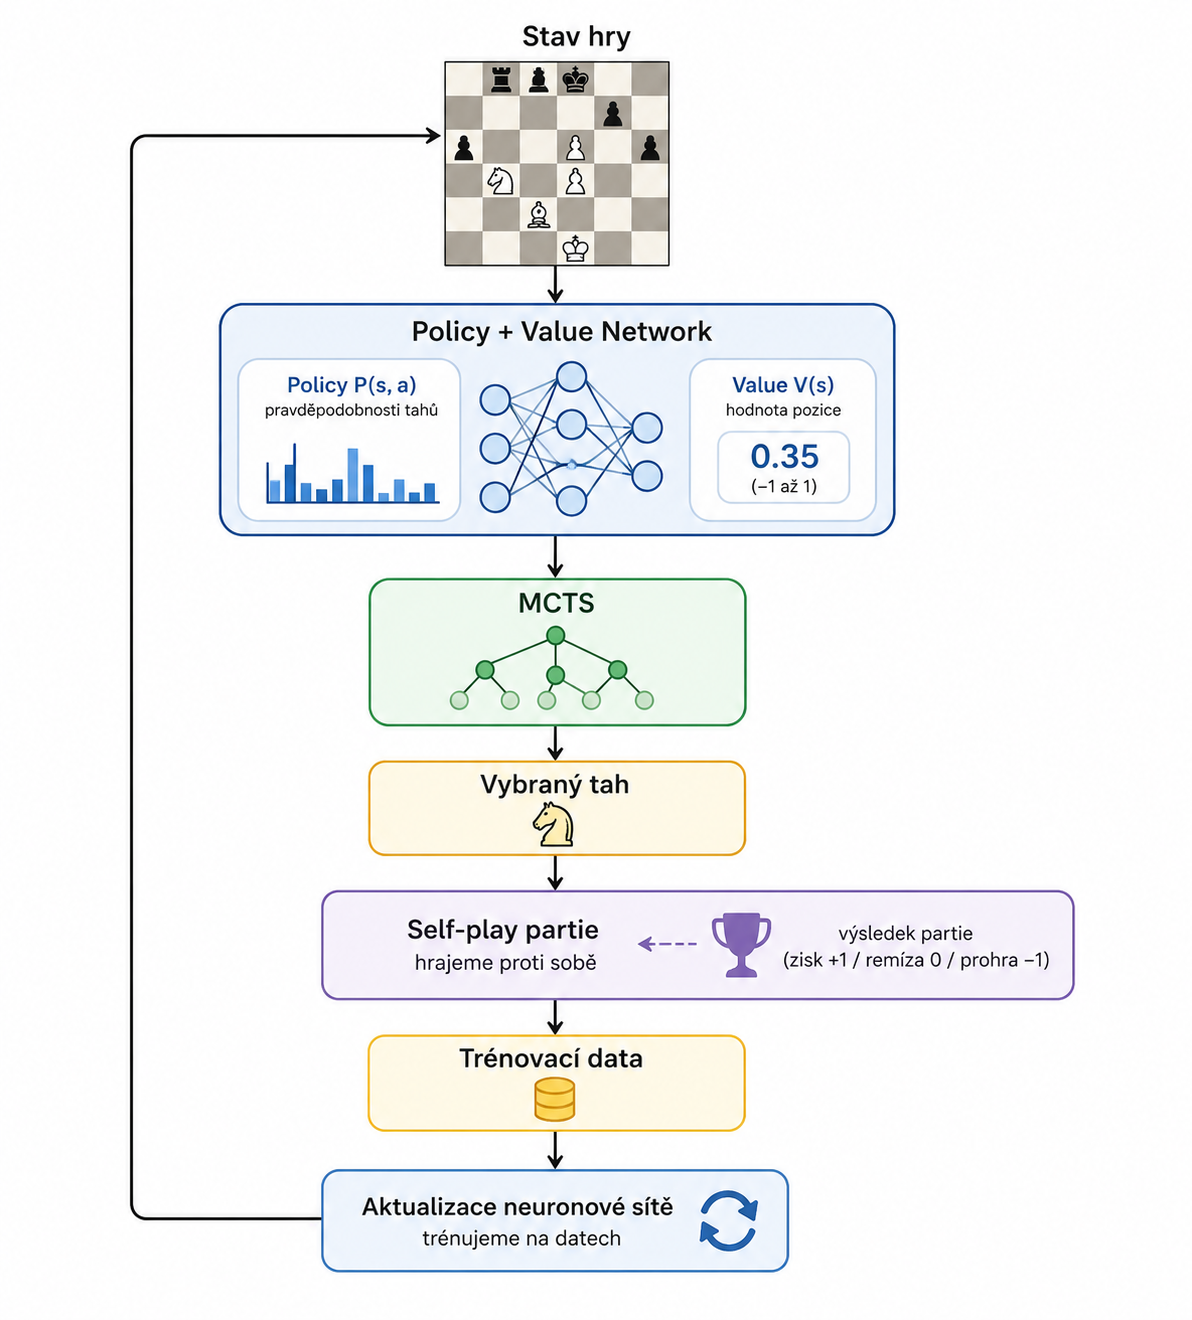
\includegraphics[width=0.85\textwidth]{img/AlphaZero.png}
    \caption{Schéma principu algoritmu AlphaZero. Obrázek vytvořen autorem na základě \cite{silver2017alphazero}.}
    \label{fig:alphazero_pipeline}
\end{figure}

\section{Self-play a trénování}

Algoritmy založené na neuronových sítích vyžadují velké množství trénovacích dat. Na rozdíl od klasických úloh strojového učení však ve 
většině deskových her neexistují velká databáze optimálních partií, kterou by bylo možné využít pro učení. Moderní algoritmy proto 
využívají metodu označovanou jako self-play, při níž agent opakovaně hraje partie sám proti sobě a získaná data využívá pro 
trénování \cite{silver2017alphazero,sutton2018rl}.

\subsection{Generování trénovacích dat}

Každá partie odehraná metodou self-play vytváří množinu trénovacích vzorků. Pro každý navštívený stav jsou ukládány informace 
potřebné pro učení neuronové sítě. Typicky se jedná o reprezentaci stavu hry, pravděpodobnostní rozdělení tahů 
získané algoritmem MCTS a konečný výsledek celé partie \cite{silver2017alphazero}.

\subsection{Trénovací proces}

Po dokončení dostatečného množství partií jsou získaná data využita k aktualizaci parametrů neuronové sítě. \emph{Policy Network} 
se učí co nejlépe aproximovat pravděpodobnostní rozdělení tahů získané algoritmem MCTS, zatímco \emph{Value Network} se učí předpovídat 
skutečný výsledek partie. Trénování probíhá opakovaně střídáním fází generování nových dat a optimalizace sítě, což 
vede k postupnému zlepšování modelu \cite{silver2017alphazero}.

\subsection{Integrace s Monte Carlo Tree Search}

Neuronová síť a algoritmus MCTS tvoří vzájemně propojený celek. Neuronová síť poskytuje algoritmu MCTS předem pravděpodobnosti 
jednotlivých tahů a odhad hodnoty stávající pozice. Na základě toho MCTS vybírá tahy během self-play a současně vytváří 
nová trénovací data. Aktualizovaná neuronová síť následně umožňuje efektivnější prohledávání herního stromu, čímž vzniká zpětnovazební
proces vedoucí k postupnému zlepšování celého systému \cite{silver2017alphazero}.